%% PRL-style letter: TPS as a diagnostic for diffusion-based generative models
%% RevTeX 4-2, two-column, Physical Review Letters format

\documentclass[aps,prl,twocolumn,superscriptaddress,floatfix]{revtex4-2}

\usepackage{amsmath,amssymb,bm}
\usepackage{graphicx}
\usepackage{xcolor}
\usepackage{hyperref}
\usepackage{algpseudocode}

\begin{document}

\title{Probing Generative Protein Structure Models with Transition Path Sampling}

\author{Muhammad R.~Hasyim}
\affiliation{Simons Center for Computational Physical Chemistry,
New York University, New York, NY~10003}
\email{mh7373@nyu.edu}

\date{\today}

\begin{abstract}
Diffusion-based structure generators sample protein conformations by reversing
a stochastic denoising process, yet the stochastic landscape underlying a
given prediction remains largely unexplored. Here we introduce a framework
that treats the reverse diffusion of Boltz-2 as a discrete-time Markov chain
on an extended state comprising coordinates, SE(3) augmentation, and per-step
Gaussian noise draws, and applies transition path sampling (TPS) to collect
statistically unbiased ensembles of denoising trajectories. Applied to a
228-residue two-chain co-folding task run without MSA information, 100 TPS
Monte Carlo steps yield an ensemble of predicted structures with C$\alpha$ RMSD
spread of only $0.48$--$0.69$~\AA{} and a $\approx 53\%$ shooting acceptance
rate, revealing that the model's stochastic landscape is sharply concentrated
near a single structural attractor. The approach provides a principled
diagnostic for characterizing generative model confidence, identifying
structurally ambiguous predictions, and evaluating the physical quality of
generated structures.
\end{abstract}

\maketitle

Diffusion-based structure generators such as AlphaFold3~\cite{alphafold3},
Boltz-2~\cite{boltz2}, and RoseTTAFold All-Atom~\cite{rfaa} are now used by
millions of researchers worldwide, yet systematic evaluations reveal a
consistent pattern of fragility: confidence scores are assigned to
intrinsically disordered regions that cannot actually be predicted, with
$\approx 18\%$ of biologically functional disordered residues
hallucinated as ordered~\cite{gopalan2025}; protein--ligand co-folding methods
largely memorize training-set poses and fail sharply on novel
compounds~\cite{skrinjar2025}; and antibody--antigen docking succeeds in fewer
than $15\%$ of predictions at a single seed~\cite{hitawala2025}.  At the scale
of millions of users, a few-percent error rate is no longer a rare edge case —
it is millions of structurally incorrect predictions entering drug pipelines
and structural databases every year.  The root diagnostic question is whether a
model has genuinely learned the physical principles of folding or merely
memorizes training-set attractors that score well on held-out benchmarks.

What is needed is a diagnostic tool that probes the full distribution of
structures a model can produce for a fixed input, rather than accepting a
single forward pass at face value.  A physics-learner should yield a sharply
focused, energetically reasonable ensemble for a stable fold and a diffuse one
for a disordered or multi-basin sequence; a memorizer will do neither
reliably.  Rare-event sampling offers exactly this probe: Dorman
et al.~\cite{dorman2026} recently applied transition path sampling (TPS) with
Metropolis--Hastings acceptance and umbrella sampling to large language models,
showing that path ensemble methods reveal failure modes entirely invisible to
direct sampling.  Here we take the same approach for protein structure
diffusion, recasting the reverse diffusion of Boltz-2 as an explicit
stochastic dynamical system and applying
TPS~\cite{dellago1998,bolhuis2002} to collect an unbiased ensemble of
denoising trajectories connecting disordered (high-$\sigma$) to structured
(low-$\sigma$) states.  The key insight is that each denoising step is driven
by explicit, computable noise draws, so the full path probability factorizes
analytically and TPS acceptance ratios are exact.

\section{TPS for diffusion dynamics}

We describe the algorithm generically (Fig.~\ref{alg:tps}), then specialize
to Boltz-2.  Unlike classical MD, the denoising kernel $G$ has no
time-reversal of itself, so we use a dedicated backward proposal
$q_{\mathrm{bwd}}(x_i|x_{i+1})$~\cite{buijsman2020}: invert the denoiser
map to recover $x_i^{\mathrm{noisy}}$ from $x_{i+1}$ (rescaled fixed-point
iteration~\cite{boltz2_tps_theory}), draw fresh noise to propose $x_i$.
Forward shooting (resample suffix, $\Delta=0$), backward shooting
($\Delta_{\mathrm{bwd}}$ corrects for $p_{\mathrm{fwd}}\neq q_{\mathrm{bwd}}$,
global reshuffle (fresh $x_0$ and all $\xi_i$, always accepts) together form
an ergodic move set on the reactive path
ensemble~\cite{falkner2024,buijsman2020}.

\begin{figure}[t]
\hrule\vspace{2pt}
{\footnotesize\textbf{Algorithm 1.} TPS for a Generic Non-Reversible Generative Model}
\vspace{1pt}\hrule\vspace{3pt}
\begin{algorithmic}[1]
\footnotesize
\Require $G$: forward kernel; $\pi_i$: noise prior; $A,B$: state volumes;
         $\mathcal{X}^{(0)}$: initial reactive path with $x_0\!\in\!A$, $x_L\!\in\!B$.
\For{$k = 1, \ldots, N_{\mathrm{MC}}$}
  \State \textbf{Select:} $i^* \sim \mathrm{Uniform}\{1,\ldots,L\!-\!1\}$
  \State \textbf{Resample:} $\xi_{i^*}^{\mathrm{new}} \sim \pi_{i^*}$;\; draw $\xi_i^{\mathrm{new}}\!\sim\!\pi_i$ for $i>i^*$
  \State \textbf{Integrate:} $x_{i+1}^{\mathrm{new}} = G(x_i^{\mathrm{new}}, \xi_i^{\mathrm{new}})$\; for $i=i^*,\ldots,L\!-\!1$
  \State \textbf{Reactivity:} if $x_L^{\mathrm{new}}\!\notin\!B$: reject, $\mathcal{X}^{(k)}\!=\!\mathcal{X}^{(k-1)}$; continue
  \State \textbf{Log-ratio:} compute $\Delta$ via Eq.~(\ref{eq:delta})
  \State \textbf{Accept:} $\mathcal{X}^{(k)}\!=\!\mathcal{X}^{\mathrm{new}}$ w.p.\ $\min(1,e^{\Delta})$; else $\mathcal{X}^{(k-1)}$
\EndFor
\end{algorithmic}
\vspace{1pt}\hrule\vspace{2pt}
{\footnotesize\textit{Note.}  The algorithm shows \emph{forward shooting} (suffix resampled,
prefix fixed, $\Delta = 0$ always).  The ergodic scheme also uses
\emph{backward shooting} (prefix via $q_{\mathrm{bwd}}$, Hastings-corrected,
Eq.~\ref{eq:deltabwd}) and \emph{global reshuffle} (fresh $x_0 \sim \rho$
and all $\xi_i$; always accepts, $\Delta = 0$).
Jacobian $\log|\det J_i|$ is trivial for i.i.d.\ noise, non-trivial for
EDM schedules.}
\vspace{1pt}
\label{alg:tps}
\end{figure}

The Boltz-2 reverse sampler advances a coordinate tensor
$x \in \mathbb{R}^{M \times 3}$ (with $M$ padded atoms) along a fixed schedule
of noise levels $\sigma_0 > \sigma_1 > \cdots > \sigma_L = 0$ over $L$
denoising steps.  We track the \emph{extended state}
$\mathcal{S}_i = (x_i, R_i, \tau_i, \varepsilon_i)$, where $R_i \in
\mathrm{SO}(3)$ and $\tau_i \sim \mathcal{N}(0, s_\tau^2 I)$ are the SE(3)
augmentation drawn at each step, and $\varepsilon_i \sim \mathcal{N}(0, v_i I)$
is the injected Gaussian noise with variance $v_i = \eta^2(\hat{t}^2 -
\sigma_i^2)$ set by the EDM schedule~\cite{karras2022}.  One complete
denoising step maps $\mathcal{S}_i \to x_{i+1}$ via
%
\begin{align}
\tilde{x}_i &= R_i\,(x_i - \bar{x}_i) + \tau_i , \label{eq:aug} \\
x_i^{\mathrm{noisy}} &= \tilde{x}_i + \varepsilon_i , \label{eq:inject} \\
x_{i+1} &= x_i^{\mathrm{noisy}}
  + s\,\frac{\sigma_i^t - \hat{t}}{\hat{t}}\,
  \frac{x_i^{\mathrm{noisy}} - \hat{x}_i}{\hat{t}} , \label{eq:update}
\end{align}
%
where $\bar{x}_i$ is the mass-weighted centroid, $\hat{x}_i = c_\mathrm{skip}
x_i^\mathrm{noisy} + c_\mathrm{out} f_\theta(c_\mathrm{in}
x_i^\mathrm{noisy}, \cdot)$ is the preconditioned denoiser output, and $s$ is a
step-scale factor.  Because each step is a \emph{deterministic} function of the
random draw $(R_i, \tau_i, \varepsilon_i)$, the joint density of a full path
$\mathcal{X} = \{(x_i, R_i, \tau_i, \varepsilon_i)\}_{i=0}^{L-1} \cup \{x_L\}$
factorizes as
%
\begin{equation}
\log P(\mathcal{X}) = \log\rho(x_0)
  + \sum_{i=0}^{L-1}\left[
    -\frac{\|\varepsilon_i\|^2}{2v_i}
    - \frac{\|\tau_i\|^2}{2s_\tau^2}
    + \log|\det J_i|
  \right],
\label{eq:logpath}
\end{equation}
%
where $\rho(x_0) \propto \mathcal{N}(0,\sigma_0^2 I)$ is the initial noise
prior, and $\log|\det J_i| = 3M \log|1 + s(\sigma_i^t - \hat{t})/\hat{t}|$ is
the per-step Jacobian arising from the affine map $\varepsilon_i \to
x_{i+1}$~\cite{boltz2_tps_theory}.  The Haar term for $R_i$ is constant and
drops from acceptance ratios.  State volumes are defined on the diffusion
coordinate: A at high $\sigma$ (disordered) and B at low $\sigma$ (structured),
so every accepted path is a complete denoising trajectory.

A forward shooting move at frame $i^*$ resamples all noise variables
$(\xi_i)_{i \geq i^*}$ and forward-integrates from that point, leaving the
prefix $(x_0, \ldots, x_{i^*})$ unchanged.  The Metropolis--Hastings
log-ratio follows directly from the factorization in Eq.~(\ref{eq:logpath}):
%
\begin{equation}
\Delta = \sum_{i \geq i^*}
  \left[
    \log\frac{\pi_i(\xi_i^{\mathrm{new}})}{\pi_i(\xi_i^{(k-1)})}
    + \log\frac{|\det J_i^{\mathrm{new}}|}{|\det J_i^{(k-1)}|}
  \right] .
\label{eq:delta}
\end{equation}
%
The proposed path is accepted with probability $\min(1,e^{\Delta})$.
Backward shooting at $k$ uses the Hastings-corrected ratio
$\Delta_{\mathrm{bwd}} = [\log\pi_{\mathrm{fwd}}(X'_{0:k}) -
\log\pi_{\mathrm{fwd}}(X_{0:k})] + [\log q_{\mathrm{bwd}}(X_{0:k}) -
\log q_{\mathrm{bwd}}(X'_{0:k})] + \log\rho(x_0')/\rho(x_0)$,
with $q_{\mathrm{bwd}}$ Gaussian in the backward noise~\cite{falkner2024}.

\section{Results}

We apply the framework to a 228-residue two-chain heterodimer using the
Boltz-2 multimer co-folding pipeline with MSA information withheld.
The system comprises $M = 1792$ padded atoms,
$L = 32$ denoising steps, and initial noise scale $\sigma_0 = 2560$~\AA.
An initial reactive trajectory is obtained from a single forward pass; TPS
then runs 100 shooting MC steps using OpenPathSampling~\cite{ops},
with acceptance evaluated via Eq.~(\ref{eq:delta}).

The shooting acceptance rate is $\approx 53\%$, consistent with a well-tuned
shooting distribution~\cite{bolhuis2002}, and all accepted paths remain
reactive.  At every 10 MC steps, we extract the final denoised structure from
the accepted path and evaluate two diagnostics: (i) C$\alpha$ RMSD with respect
to the initial accepted structure, and (ii) the total potential energy computed
by energy minimization in OpenMM.  The resulting TPS ensemble of 10 structures
is shown in Fig.~\ref{fig:structures}.

The C$\alpha$ RMSD values across the ensemble span only $0.48$--$0.69$~\AA{}
with mean $0.59 \pm 0.06$~\AA{} (Fig.~\ref{fig:distributions}a), indicating
that TPS consistently produces structures within sub-angstrom deviation of one
another.  The OpenMM energy ranges from $-42{,}201$ to $-41{,}653$~kJ/mol, a
spread of $548$~kJ/mol, with all structures converging to physically reasonable
configurations (Fig.~\ref{fig:distributions}b).  The narrow RMSD distribution
is not a failure of the shooting moves to explore the stochastic space: each
accepted path involves entirely different random draws
$(R_i, \tau_i, \varepsilon_i)$ at every denoising step, so the structural
similarity is a genuine property of the model's denoising landscape rather than
a sampling artifact.

\begin{figure}[t]
  \centering
  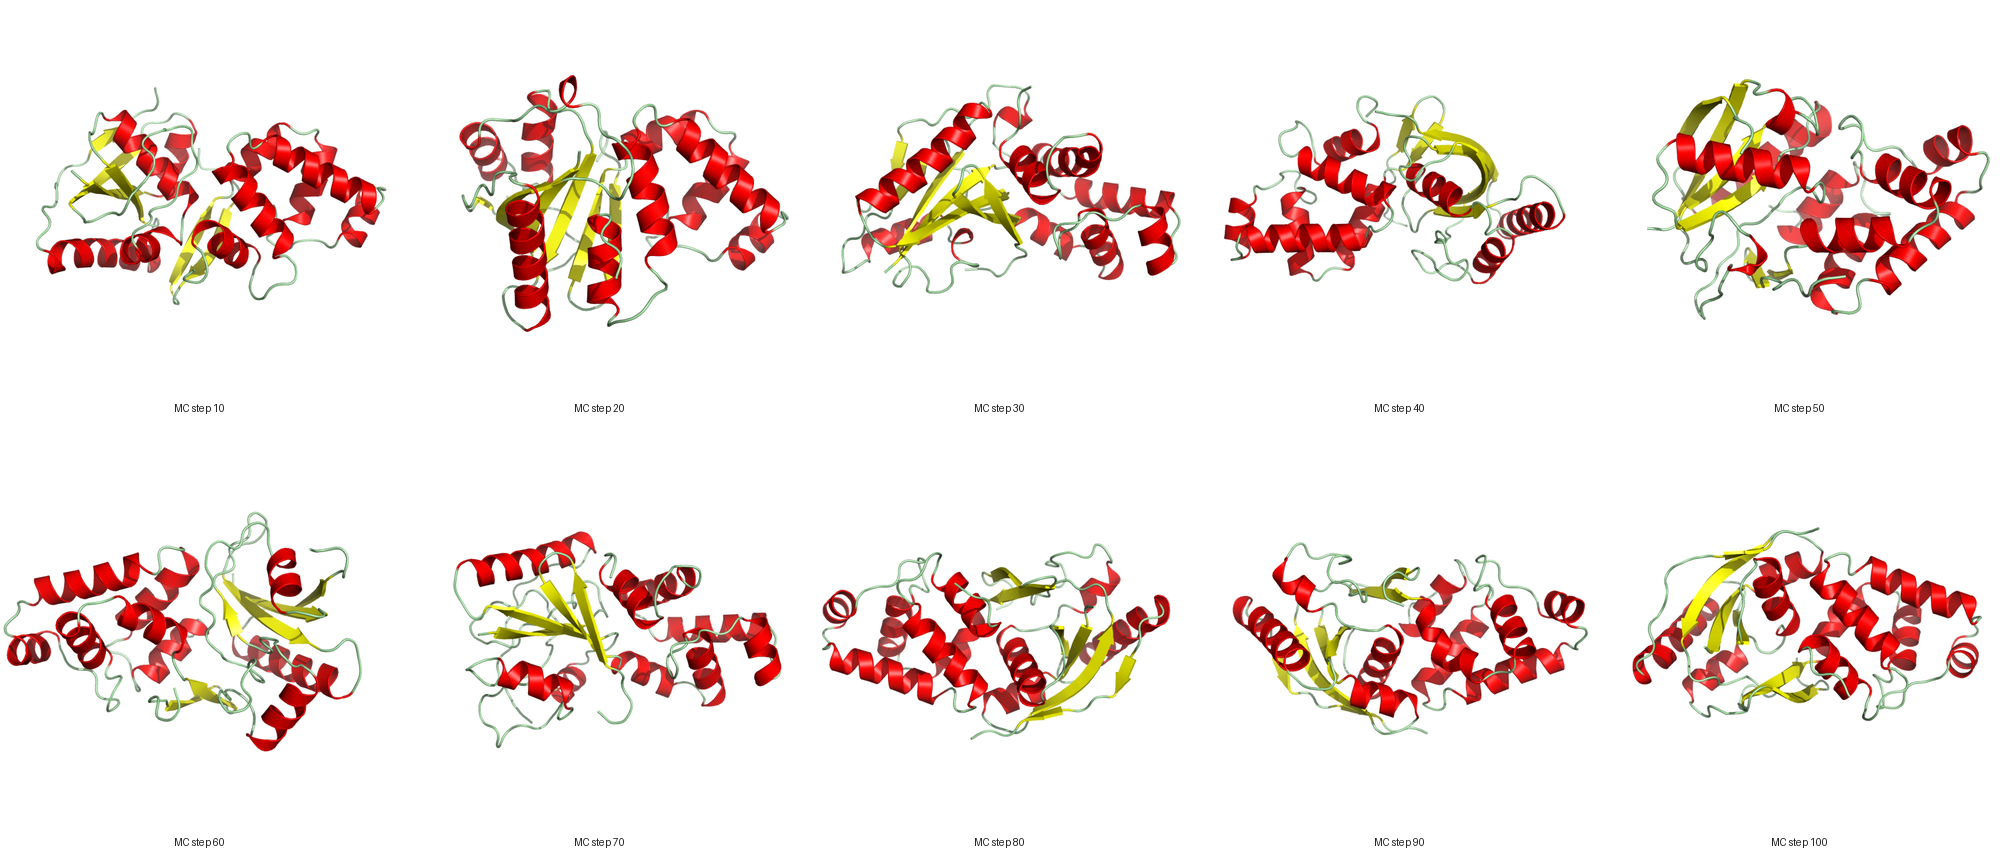
\includegraphics[width=\columnwidth]{../cofolding_tps_out_fixed/checkpoint_last_frames_grid.png}
  \caption{\textbf{TPS-sampled structural ensemble.}
  Final denoised structures extracted from 10 consecutive accepted TPS paths
  (MC steps 10--100 in increments of 10), rendered as C$\alpha$ ribbon
  cartoons.  Both chains of the heterodimer are shown; chain coloring is
  preserved across panels.  The overall fold and interface geometry are
  consistent across the ensemble, with the largest variations confined to
  exposed loop regions.  The visual similarity is quantified in
  Fig.~\ref{fig:distributions}.
  }
  \label{fig:structures}
\end{figure}

\section{Discussion}

The tight RMSD distribution reflects a sharply funneled denoising landscape:
despite stochastic freedom at every step, the model converges to the same
structure from a wide range of intermediate noise configurations.  A model
uncertain about the correct fold would exhibit a broad RMSD distribution; one
that is overfit would show an unnaturally narrow distribution with unphysically
low energy variance.  The combination of structural and energetic distributions
thus provides a two-dimensional fingerprint of generative model behavior.

This perspective elevates TPS from a rare-event method into a general-purpose
diagnostic.  The framework applies to any generator that can be cast as an
explicit Markov chain with computable transition kernels, including score-based
diffusion, flow matching, and closely related
architectures~\cite{song2021,lipman2022}. TPS requires only that path weights
are computable — satisfied here by Eq.~(\ref{eq:logpath})~\cite{falkner2023}
— and shifts the question from ``what structures does the model produce on
average'' to ``what is the full reactive ensemble for this specific input''.
The full ergodic move set (forward + backward shooting + global reshuffle)
ensures the Markov chain on the reactive path ensemble is irreducible
regardless of the connectivity of path
space~\cite{falkner2024,buijsman2020}.

\begin{figure}[t]
  \centering
  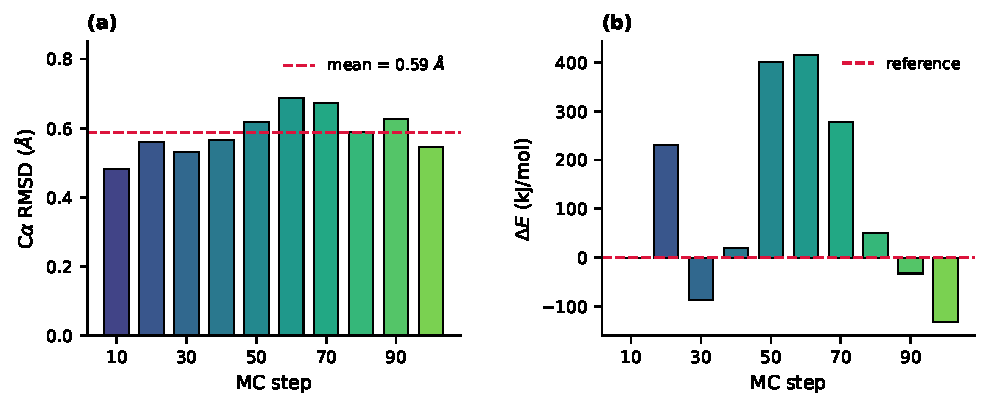
\includegraphics[width=\columnwidth]{fig_distributions_placeholder.pdf}
  \caption{\textbf{Structural and energetic distributions of the TPS ensemble.}
  (a) C$\alpha$ RMSD values of each accepted checkpoint structure relative to the
  first TPS-accepted structure, for 10 structures sampled at MC steps
  10--100.  The distribution is narrow ($0.48$--$0.69$~\AA, mean
  $0.59 \pm 0.06$~\AA), indicating strong structural convergence across
  distinct denoising trajectories.
  (b) Total potential energy (kJ/mol) evaluated by OpenMM energy minimization
  for each TPS checkpoint structure.  All structures fall in the range
  $-42{,}201$ to $-41{,}653$~kJ/mol with a spread of $\approx 548$~kJ/mol,
  confirming that TPS-sampled structures are physically reasonable across the
  ensemble.
  }
  \label{fig:distributions}
\end{figure}

Several directions follow naturally.  Applying TPS across MSA depths would
directly quantify how evolutionary information focuses the model's stochastic
landscape.  For disordered or multi-basin proteins a broad TPS ensemble would
serve as an early warning against over-interpreting the single-best prediction.
The path weights in Eq.~(\ref{eq:logpath}) can further be used to compute
free-energy-like averages over structural order parameters without any
modification of the model itself.

In summary, we show that the reverse diffusion of Boltz-2 admits a rigorous
TPS formulation on an extended state that includes SE(3) augmentation and
per-step noise draws, that the resulting path probability factorizes cleanly,
and that 100 MC steps are sufficient to characterize the model's stochastic
landscape for a 228-residue co-folding task.  The sub-angstrom structural
spread we find establishes that the model is highly confident in its prediction
for this input, and the framework provides a direct route to interrogating
generative model behavior in cases where confidence is less clear.

\begin{acknowledgments}
The author acknowledges support from the Simons Center for Computational
Physical Chemistry (SCCPC) at New York University (SF Grant No.~839534) and
the use of NYU IT High Performance Computing resources.
\end{acknowledgments}

\begin{thebibliography}{99}

\bibitem{dorman2026}
J.~M.~Dorman, E.~Gillman, D.~C.~Rose, J.~F.~Mair, and J.~P.~Garrahan,
Rare event analysis of large language models,
\textit{arXiv:2602.06791} (2026).

\bibitem{gopalan2025}
S.~Gopalan and S.~Narayanan,
Hallucinations in AlphaFold3 for intrinsically disordered proteins with
disorder in biological process residues,
\textit{arXiv:2510.15939} (2025).

\bibitem{skrinjar2025}
P.~\v{S}krinjar, J.~Eberhardt, G.~Tauriello, T.~Schwede, and J.~Durairaj,
Have protein-ligand cofolding methods moved beyond memorisation?
\textit{bioRxiv} (2025), \url{https://doi.org/10.1101/2025.02.03.636309}.

\bibitem{hitawala2025}
F.~N.~Hitawala and J.~J.~Gray,
What does AlphaFold3 learn about antibody and nanobody docking, and what
remains unsolved?
\textit{PMC12360200} (2025).

\bibitem{boltz2}
J.~Wohlwend, G.~Corso, S.~Passaro, M.~Reveiz, V.~Portnoi, R.~Gondal,
T.~Hothorn, R.~Barzilay, and T.~Jaakkola,
Boltz-2: Towards accurate and efficient binding affinity prediction,
\textit{bioRxiv} (2025), \url{https://doi.org/10.1101/2025.05.06.651165}.

\bibitem{alphafold3}
J.~Abramson \textit{et al.},
Accurate structure prediction of biomolecular interactions with AlphaFold~3,
\textit{Nature} \textbf{630}, 493 (2024).

\bibitem{rfaa}
R.~Krishna \textit{et al.},
Generalized biomolecular modeling and design with RoseTTAFold All-Atom,
\textit{Science} \textbf{384}, eadl2528 (2024).

\bibitem{dellago1998}
C.~Dellago, P.~G.~Bolhuis, F.~S.~Csajka, and D.~Chandler,
Transition path sampling and the calculation of rate constants,
\textit{J.~Chem.~Phys.} \textbf{108}, 1964 (1998).

\bibitem{bolhuis2002}
P.~G.~Bolhuis, D.~Chandler, C.~Dellago, and P.~L.~Geissler,
Transition path sampling: Throwing ropes over rough mountain passes, in the dark,
\textit{Annu.~Rev.~Phys.~Chem.} \textbf{53}, 291 (2002).

\bibitem{karras2022}
T.~Karras, M.~Aila, S.~Laine, and J.~Lehtinen,
Elucidating the design space of diffusion-based generative models,
\textit{Adv.~Neural Inf.~Process.~Syst.} \textbf{35}, 26565 (2022).

\bibitem{boltz2_tps_theory}
M.~R.~Hasyim,
Transition Path Sampling for Boltz-2 Reverse Diffusion: Extended State Space,
Kernels, and Discrete-Time TPS,
unpublished notes (2025).

\bibitem{song2021}
Y.~Song, J.~Sohl-Dickstein, D.~P.~Kingma, A.~Kumar, S.~Ermon, and B.~Poole,
Score-based generative modeling through stochastic differential equations,
\textit{ICLR} (2021).

\bibitem{lipman2022}
Y.~Lipman, R.~T.~Q.~Chen, H.~Ben-Hamu, M.~Nickel, and M.~Le,
Flow matching for generative modeling,
\textit{ICLR} (2023).

\bibitem{falkner2024}
S.~Falkner, A.~Coretti, B.~G.~Peters, P.~G.~Bolhuis, and C.~Dellago,
Revisiting shooting point Monte Carlo methods for transition path sampling,
\textit{J.~Chem.~Phys.}, arXiv:2408.03054 (2024).

\bibitem{buijsman2020}
P.~Buijsman and P.~G.~Bolhuis,
Transition path sampling for non-equilibrium dynamics without predefined
reaction coordinates,
\textit{J.~Chem.~Phys.} \textbf{152}, 044107 (2020).

\bibitem{falkner2023}
S.~Falkner, A.~Coretti, S.~Romano, P.~Geissler, and C.~Dellago,
Conditioning Boltzmann generators for rare event sampling,
\textit{Mach.~Learn.: Sci.~Technol.} \textbf{4}, 035050 (2023).

\bibitem{ops}
D.~W.~Swenson, J.-H.~Prinz, F.~Noé, J.~D.~Chodera, and P.~G.~Bolhuis,
OpenPathSampling: A Python framework for path sampling simulations.
1.~Basics,
\textit{J.~Chem.~Theory Comput.} \textbf{15}, 813 (2019).

\end{thebibliography}

\end{document}
